% This work is licensed under the Creative Commons
% Attribution-NonCommercial-ShareAlike 4.0 International License. To view a copy
% of this license, visit http://creativecommons.org/licenses/by-nc-sa/4.0/ or
% send a letter to Creative Commons, PO Box 1866, Mountain View, CA 94042, USA.
\section{Aufgabenblatt 9}
\subsection*{Aufgabe $\ast$)}
\begin{itemize}
	\item deterministischer endlicher Automat: ist ein NEA mit
	\begin{align*}
		\forall q\in Q,\forall a\in\Sigma:\exists! q'\in Q:(q,a,q')\in\Delta
	\end{align*}
	\item Potenzmengenkonstruktion: siehe letztes Übungsblatt.
	\item erreichbarer Zustand: Ein Zustand $q\in Q$ heißt \textbf{erreichbar}
	\begin{align*}
		:\Longleftrightarrow\exists w\in\Sigma^\ast:\delta(q_0,w)=q
	\end{align*}
	\item äquivalente Zustände: Sei $\A=(Q,\Sigma,q_0,\delta,F)$ ein DEA. 
	Für $q\in Q$ sei $\A_q:=(Q,\Sigma,q,\delta,F)$. 
	Zwei Zustände $q,q'\in Q$ heißen \textbf{äquivalent}, i.Z. 
	\begin{align*}
		q\sim_\A q':\Longleftrightarrow L(\A_q)=L(\A_{q'})
	\end{align*}
	\item Quotientenautomat: Der \textbf{Quotientenautomat} 
	$\tilde{\A}=(\tilde{Q},\Sigma,\tilde{q}_0,\tilde{\delta},\tilde{F})$ zu\\ $\A=(Q,\Sigma,q_0,\delta,F)$ ist definiert durch
	\begin{itemize}
		\item $\tilde{Q}:=\lbrace[q]_\sim\mid q\in Q\rbrace$
		\item $\tilde{\delta}([q]_\sim,a):=[\delta(q,a)]_\sim=:\widetilde{\delta(q,a)}$
		\item $\tilde{F}:=\lbrace[q]_\sim\mid q\in F\rbrace$
	\end{itemize}
	\item reduzierter Automat: Für einen DEA $\A$ bezeichnet $\A_{\text{red}}:=\tilde{\A}_0$ den 	\textbf{reduzierten Automaten}, den man aus $\A$ durch Eliminieren unerreichbarer Zustände und Zusammenfassen äquivalenter Zustände erhält.
	\item Nerode-Rechtskongruenz: Sei $L\subseteq\Sigma^\ast$ eine beliebige Sprache. 
	Für $u,v\in\Sigma^\ast$ definieren wir:
	\begin{align*}
		u\cong_L v:\Longleftrightarrow\forall w\in\Sigma^\ast:uw\in L\Leftrightarrow vw\in L
	\end{align*}
	``Egal was man hinten anhängt, sie verhalten sich bzgl. der Sprache gleich.''
\end{itemize}

\subsection*{Aufgabe $\ast\ast$)}
\subsubsection*{Aufgabe $\ast\ast$) (a)}
%TODO

%\usetikzlibrary{positioning,automata}
%\begin{tikzpicture}[shorten >=1pt,node distance=2.7cm,on grid]
%  \node[state,initial]   (q_0)                {$q_0$};
%  \node[state]           (q_1) [right=of q_0] {$q_1$};
%  \node[state,accepting] (q_2) [right=of q_1] {$q_2$};
%  \path[->] (q_0) edge                node [above] {a} (q_1)
%            (q_1) edge [loop above]   node [above] {a,b} ()
%                  edge                node [above] {a} (q_2);
%\end{tikzpicture}

\subsubsection*{Aufgabe $\ast\ast$) (b)}
%TODO

%\usetikzlibrary{positioning,automata}
%\begin{tikzpicture}[shorten >=1pt,node distance=2.7cm,on grid]
%  \node[state,initial, accepting]   (q_0)                {$q_0$};
%  \node[state]           (q_1) [above right=of q_0] {$q_1$};
%  \node[state] (q_2) [below right=of q_0] {$q_2$};
%  \node[state] (q_3) [above right=of q_2] {$q_3$};
%  \path[->] (q_0) edge [bend left=30] node [above] {a} (q_1)
%                  edge [bend left=30] node [above] {b} (q_2)
%            (q_1) edge [bend left=30] node [above] {a} (q_0)
%            	  edge [bend left=30] node [above] {b} (q_3)
%            (q_2) edge [bend left=30] node [above] {b} (q_0)
%                  edge [bend left=30] node [above] {a} (q_3)
%            (q_3) edge [bend left=30] node [above] {b} (q_1)
%                  edge [bend left=30] node [above] {a} (q_2);
%\end{tikzpicture}

\subsection{Aufgabe 1}

\textbf{Wiederholung:} Approximation $\sim_k$ von $\sim_\A$:
\begin{itemize}
	\item $q\sim_0 q':\Longleftrightarrow (q\in F\Leftrightarrow q'\in F)$
	\item $q\sim_{k+1} q':\Longleftrightarrow(q\sim_k q\wedge\forall a\in\Sigma:\delta(q,a)\sim_k\delta(q',a)$
\end{itemize}
In Aufgabe 8.4 (b) wurde gezeigt:
\begin{align*}
	(\exists k\in\N:\sim_k=\sim_{k+1})\implies\sim_k=\sim_\A
\end{align*}
Bestimme also $\sim_\A$ schrittweise durch Approximation:
\begin{itemize}
	\item $Q/_{\sim_0}=\big\lbrace\lbrace q_1,q_2,q_4\rbrace,\lbrace q_0,q_3,q_5\rbrace\big\rbrace$ Wir trennen also die Endzustände von den Nichtendzuständen (dies ist immer der erste Schritt). Nun ``verfeinern'' wir diese Zerlegung.
	\item $Q/_{\sim_1}=\big\lbrace\lbrace q_1,q_2,q_4\rbrace,\lbrace q_0,q_3,\rbrace,\lbrace q_5\rbrace\big\rbrace$ (``Bleibt $q_i$ in der Äquivalenzklasse?'')
	\item $Q/_{\sim_2}=\big\lbrace\lbrace q_1,q_2,q_4\rbrace,\lbrace q_0,q_3\rbrace,\lbrace q_5\rbrace\big\rbrace=Q|_{\sim_1}\implies \sim_2=\sim_1=\sim_\A$ 
\end{itemize}

Mit $\tilde{q}:=[q|_{\sim_\A}=\lbrace q'\in Q\mid  q\sim_\A g'\rbrace$ erhalten wir:
\begin{align*}
	\tilde{A}&=\big(\lbrace\tilde{q}_1,\tilde{q}_0,\tilde{q}_5\rbrace,\lbrace a,b\rbrace,\tilde{q}_0,\tilde{\delta},
	\underbrace{\lbrace\tilde{q}_1,\tilde{q}_2,\tilde{q}_4\rbrace}_{=\lbrace\tilde{q}_1\rbrace}\big)\mit\\
	\tilde{\delta}(\tilde{q},x)&:=\widetilde{\delta(q,x)}\mit x\in\lbrace a,b\rbrace
\end{align*}

Quotientenautomat $\tilde{\A}$:
\usetikzlibrary{positioning,automata}
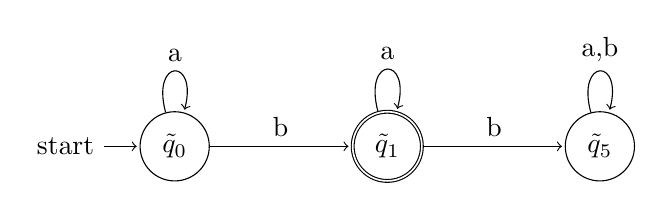
\begin{tikzpicture}[shorten >=1pt,node distance=2.7cm,on grid]
  \node[state,initial]   (q_0)                {$\tilde{q}_0$};
  \node[state, accepting](q_1) [right=of q_0] {$\tilde{q}_1$};
  \node[state] (q_5) [right=of q_1] {$\tilde{q}_5$};
  \path[->] (q_0) edge [loop above] node [above] {a} ()
                  edge [bend left=0] node [above] {b} (q_1)
            (q_1) edge [loop above] node [above] {a} ()
            	  edge [bend left=0] node [above] {b} (q_5)
            (q_5) edge [loop above] node [above] {a,b} ();
\end{tikzpicture}

\subsection{Aufgabe 2}


Der Vorlesung folgend bezeichne $\A_0$ den zu $\A$ äquivalenten Automaten, den man erhält, indem man alle in $\A$ unerreichbaren Zustände entfernt (und $\delta$ entsprechend anpasst oder einschränkt). 
Hier entspricht $\A_0$ also $\A$ ohne $q_8$.\nl
Nun berechnen wir den Quotientenautomaten $\tilde{\A}_0$ von $\A_0$.\\
Bestimme zuerst $\tilde{\A}_0$: ($Q=\lbrace q_0,\ldots,q_7\rbrace$!)
\begin{itemize}
	\item $Q/_{\sim_0}=\big\lbrace q_3,q_6\rbrace,\lbrace q_0,q_1,q_2,q_4,q_5,q_7\rbrace\big\rbrace$
	\item $Q|_{\sim_1}=\big\lbrace q_3\rbrace,\lbrace q_6\rbrace,\lbrace q_0,q_1,q_7\rbrace,\lbrace q_2\rbrace,\lbrace q_4,q_5\rbrace\big\rbrace$
	\item $Q/_{\sim_2}=\big\lbrace q_3\rbrace,\lbrace q_6\rbrace,\lbrace q_0\rbrace,\lbrace q_1\rbrace,\lbrace q_7\rbrace,\lbrace q_2\rbrace,\lbrace q_4\rbrace,\lbrace q_5\rbrace\big\rbrace$
	\item $Q/_{\sim_3}=Q|_{\sim_2}\implies\sim_3=\sim_2=\sim_{\A_0}$
\end{itemize}
Hier sind also alle Zustände paarweise nicht äquivalent zueinander. 
Der zu $\A$ reduzierte DEA $\A_{\text{red}}$ ist also:
\begin{align*}
	\A_{\text{red}}=\tilde{\A}_0\cong\A_0
\end{align*}
Das heißt, also $\tilde{\A}_0$ isomorph zu $\A_0$ ist (also gleich bis auf Umbenennung der Zustände). Also im Prinzip ist gar nichts passiert (außer, dass $q_8$ entfernt wurde).

\subsection{Aufgabe 3}
Diese Aufgabe zeigt, warum es trotzdem sinnvoll sein kann, Nicht-DEAs zu verwenden.

\subsubsection{Aufgabe 3 a)}
\begin{align*}
	L(\A_n)
	&=\big\lbrace q\in\lbrace a,b\rbrace^\ast\mid\text{der $n$-te Buchstabe von hinten in $w$ ist ein }a\big\rbrace\\
	&=\lbrace a,b\rbrace^\ast\cdot\lbrace a\rbrace\cdot\lbrace a,b\rbrace^{n-1}
\end{align*}

\subsubsection{Aufgabe 3 b)}
$\A_3$:\\
\usetikzlibrary{positioning,automata}
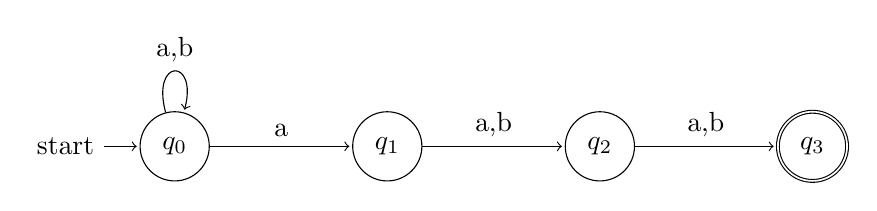
\begin{tikzpicture}[shorten >=1pt,node distance=2.7cm,on grid]
  \node[state,initial]   (q_0)                {$q_0$};
  \node[state](q_1) [right=of q_0] {$q_1$};
  \node[state] (q_2) [right=of q_1] {$q_2$};
  \node[state, accepting] (q_3) [right=of q_2] {$q_3$};
  \path[->] (q_0) edge [loop above] node [above] {a,b} ()
                  edge [bend left=0] node [above] {a} (q_1)
            (q_1) edge [bend left=0] node [above] {a,b} (q_2)
            (q_2) edge [bend left=0] node [above] {a,b} (q_3);
\end{tikzpicture}

Berechnung eines äquivalenten DEA $\A_3'$ durch Potenzmengenkonstruktion: (Bild müsste mal hier rein geteXt werden ;)
%TODO tikz-Bild

Umbenennung der Zustände des Quotientenautomaten:
\begin{itemize}
	\item $p_0:=\lbrace q_0\rbrace$
	\item $p_1:=\lbrace q_0,q_1\rbrace$
	\item $p_2:=\lbrace q_0,q_1,q_2\rbrace$
	\item $p_3:=\lbrace q_0,q_2\rbrace$
	\item $p_4:=\lbrace q_0,q_1,q_2,q_3\rbrace$
	\item $p_5:=\lbrace q_0,q_2,q_3\rbrace$
	\item $p_6:=\lbrace q_0,q_1,q_3\rbrace$
	\item $p_7:=\lbrace q_0,q_3\rbrace$
\end{itemize}

Berechnung des Quotientenautomaten (nach Konstruktion gibt es keine unerreichbaren Zustände in obiger Potenzmengenkonstruktion):
\begin{itemize}
	\item $Q/_{\sim_0}=\big\lbrace\lbrace p_4,p_5,p_6,p_7\rbrace,\lbrace p_0,p_1,p_2,p_3\rbrace\big\rbrace$
	\item $Q/_{\sim_1}=\big\lbrace\lbrace p_4,p_5\rbrace,\lbrace p_6,p_7\rbrace,\lbrace p_0,p_1\rbrace,\lbrace p_2,p_3\rbrace\big\rbrace$
	\item $Q/_{\sim_2}=\big\lbrace\lbrace p_4\rbrace,\lbrace p_5\rbrace,\lbrace p_6\rbrace,\lbrace p_7\rbrace,\lbrace p_0\rbrace,\lbrace p_1\rbrace,\lbrace p_2\rbrace,\lbrace p_3\rbrace\big\rbrace=Q|_{\sim_3}\implies\sim_2=\sim_3=\sim_{\A'}$
\end{itemize}
Daher gilt: $\A_3\cong(\A_3')_{\text{red}}$ (analog zu Aufgabe 2).

\subsubsection{Aufgabe 3 c)}
Seien also $x=x_1 x_2\hdots x_n\in\lbrace a,b\rbrace^n$ und $y=y_1 y_2\hdots y_n\in\lbrace a,b\rbrace^n$ mit $x\neq y$.\\
Zu zeigen: $x\not\cong_{L(\A_n)} y$, d.h.
\begin{align*}
	\exists w\in\lbrace a,b\rbrace^\ast:\big(xw\in L(\A_n)\wedge yw\not\in L(\A_n)\big)\vee\big(xw\not\in L(\A_n)\wedge yw\in L(\A_n)\big)
\end{align*}
Da $x\neq y$, gibt es einen kleinsten Index $j\in\lbrace1,\ldots,n\rbrace$ so, dass $x_j\neq y_j$ (die erste Position von links, an der sich $x$ und $y$ unterscheiden). 
Setze dann 
\begin{align*}
	w:=a^{j-1}
\end{align*}
Dann gibt es zwei Möglichkeiten für $x_j,y_j$:
\begin{enumerate}
	\item $x_j=a$ und $y_j=b$:
	\begin{align*}
		xw&=x_1\hdots x_{j-1}\underbrace{ a x_{j+1}\hdots x_n\underbrace{a\hdots a}_{j-1\text{ viele}}}_{n-(j-1)+(j-1)=n}\in L(\A_n)\\
		yw&=y_1\hdots y_{j-1}\underbrace{ b y_{j+1}\hdots x_n\underbrace{a\hdots a}_{j-1\text{ viele}}}_{n-(j-1)+(j-1)=n}\not\in L(\A_n)
	\end{align*}
	\item $x_j=b$ und $y_j=a$: analog.
\end{enumerate}

Alle paarweise verschiedenen Worte der Länge $n$ über dem Alphabet über $\lbrace a,b\rbrace$ sind nicht äquivalent bzgl. $\cong_{L(\A_n)}$. Da es $2^n$ verschiedene Wörter über $\lbrace a,b\rbrace$ gibt, so gibt es auch mindestens $2^n$ verschiedene Äquivalenzklassen von $\cong_{L(\A_n)}$. Aus Lemma 2.15 (4) folgt damit, dass ein minimaler Automat mindestens $2^n$ Zustände hat.
